\chapter{Chapter 2 Supplementary Content}\label{app:suppcontent}
\myappendices{Appendix \ref{app:suppcontent}: Chapter 2 Supplementary Content}
\newpage

\section{The Anatomical Fiducial Protocol}\label{app:AFIDs_supp}
The full AFIDs annotation protocol which can be access on: \url{https://afids.github.io/afids-protocol}. Figure \ref{fig:figuresupall_afids} provides a snippet of all 32 AFIDs in the three cardinal anatomical planes on the MNI2009bAsym template. 

\begin{figure}[hbt!]
    \centering
    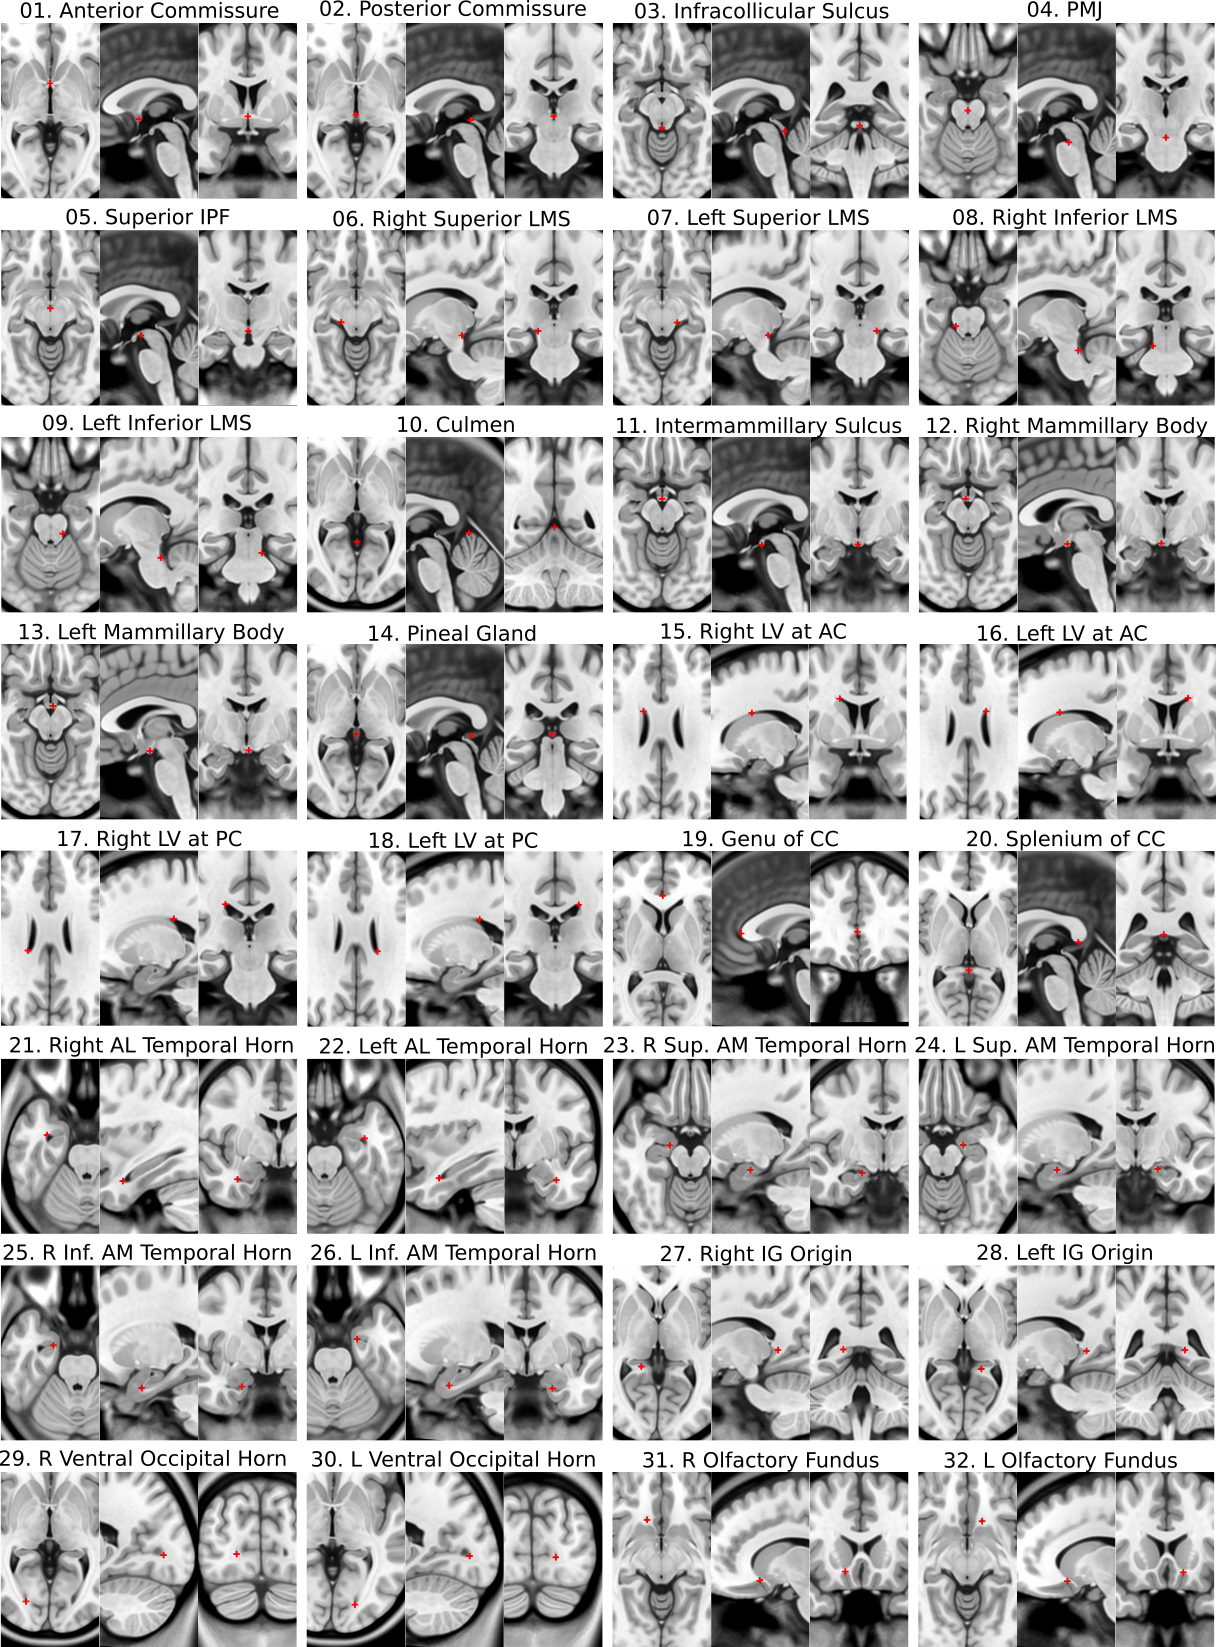
\includegraphics[width=0.8\linewidth]{figs/figuresupall_afids.png}
    \caption{The anatomical fiducials in the protocol is demonstrated with crosshairs at the representative location. AC, anterior commissure; AL, anterolateral; AM, anteromedial; IG, indusium griseum; IPF, interpeduncular fossa; LMS, lateral mesencephalic sulcus; LV, lateral ventricle; PC, posterior commissure; PMJ, pontomesenphalic junction.}
    \label{fig:figuresupall_afids}
\end{figure}


\newpage
\section{Rater Demographic Data}\label{app:rater_demo_data}
All annotations were performed by at least two human raters. As part of any annotation study, we collected demographic data on rater's experience in neuroanatomy, medical imaging, 3DSlicer software. Although not used in this paper, we also curated subthalamic nucelus (STN) segmentations on ultra-high field MRI (i.e., \(>\)7-T) data and add demographic rater data here for completeness. This data is used in Chapter \ref{chap:afidspred}. Table \ref{tab:rater_demographic_data} provides a breakdown of all the raters involved in datasets released in this work. 

\begin{table}[htbp]
\centering
\caption{
Summary of anatomical fiducial (AFID) and subthalamic nucleus (STN) annotation across datasets. Each row represents a unique annotator (Rater\_ID) contributing to one or more datasets. The table includes the experience (in months) of raters in three domains: Imaging, Neuroanatomy, and 3D Slicer. The diversity of rater backgrounds and annotation volumes reflects the breadth of participation across studies. Rater\_ID entries are context-specific and assigned uniquely within each dataset.
}
\begin{tabular}{llllll}
\toprule
Annotation & Dataset & Rater\_ID & Imaging & Neuroanatomy & 3DSlicer \\
\midrule
AFIDs & LHSCPD & AT & 0 & 0 & 0 \\
AFIDs & LHSCPD & GG & 60 & 60 & 60 \\
AFIDs & LHSCPD & MA & 60 & 60 & 60 \\
AFIDs & LHSCPD & MJ & 0 & 0 & 0 \\
AFIDs & LHSCPD & RC & 0 & 0 & 0 \\
AFIDs & AFIDs-HCP & AT & 60 & 60 & 60 \\
AFIDs & AFIDs-HCP & CZ & 12 & 12 & 12 \\
AFIDs & AFIDs-HCP & GG & 60 & 60 & 60 \\
AFIDs & AFIDs-HCP & DC & 24 & 24 & 24 \\
AFIDs & AFIDs-HCP & KF & 24 & 24 & 24 \\
AFIDs & SNSX32 & Rater01 & 12 & 12 & 12 \\
AFIDs & SNSX32 & Rater02 & 24 & 24 & 24 \\
AFIDs & SNSX32 & Rater03 & 24 & 24 & 24 \\
AFIDs & SNSX32 & Rater04 & 36 & 36 & 36 \\
AFIDs & SNSX32 & Rater05 & 24 & 24 & 24 \\
AFIDs & SNSX32 & Rater06 & 24 & 24 & 24 \\
AFIDs & SNSX32 & Rater07 & 24 & 24 & 24 \\
AFIDs & SNSX32 & Rater08 & 60 & 60 & 60 \\
AFIDs & SNSX32 & Rater09 & 12 & 12 & 12 \\
AFIDs & AFIDs-OASIS, MNI & Rater01 & 24 & 24 & 24 \\
AFIDs & AFIDs-OASIS, MNI & Rater02 & 0 & 0 & 0 \\
AFIDs & AFIDs-OASIS, MNI & Rater03 & 8 & 0 & 8 \\
AFIDs & AFIDs-OASIS, MNI & Rater04 & 24 & 6 & 0 \\
AFIDs & AFIDs-OASIS, MNI & Rater05 & 0 & 24 & 0 \\
AFIDs & AFIDs-OASIS, MNI & Rater06 & 24 & 12 & 12 \\
AFIDs & AFIDs-OASIS, MNI & Rater07 & 12 & 48 & 12 \\
AFIDs & AFIDs-OASIS, MNI & Rater08 & 0 & 0 & 0 \\
AFIDs & AFIDs-OASIS, MNI & Rater09 & 120 & 120 & 60 \\
AFIDs & 3T7T & Rater01 & 72 & 72 & 72 \\
AFIDs & 3T7T & Rater02 & 120 & 120 & 120 \\
AFIDs & 3T7T & Rater03 & 24 & 24 & 24 \\
AFIDs & 3T7T & Rater04 & 24 & 12 & 12 \\
AFIDs & 3T7T & Rater05 & 12 & 36 & 48 \\
AFIDs & 3T7T & Rater06 & 0 & 12 & 0 \\
STN & SNSX & Rater A & 120 & 120 & 60 \\
STN & SNSX & Rater B & 240 & 240 & 12 \\
STN & SNSX & Rater C & 72 & 72 & 72 \\
STN & 3T7T & Rater A & 84 & 84 & 84 \\
\bottomrule
\end{tabular}
\label{tab:rater_demographic_data}
\end{table}